\minitoc
% \startcontents[chapters]
% \printcontents[chapters]{}{1}{}

% \begin{FraseCelebre}
%     \begin{Frase}
%         In the end, I must proclaim that no good can be achieved of false means. For the substance of our existence is not in the achievement, but in the method.
%     \end{Frase}
%     \begin{Fuente}
%         Dalinar Kholin, The Way of Kings
%     \end{Fuente}
% \end{FraseCelebre}

\section{Introduction}
\label{sec:bug-hunter:intro}
%\jgb{There was \cn both for the importance of building past snapshots, and for the importance of tests. I assume both things are evident enough, and don't need a citation. However, if you feel you can include a illustrating citation, please do.}

Reproducing (building) executable programs from the source code of past snapshots
%\patxi{Ojo, usa consistentemente snapshot o commit o change en la tesis. No recuerdo cómo está en el capítulo del emse al final}\michel{En este paper, el uso es consistente. En intro y related work se habla de snapshot. En la sección de definiciones, se introduce el commit como una snapshot del código fuente}
 of a project is fundamental for practitioners, to maintain old versions still in production, and for researchers, to study those old versions. 
To our knowledge, Tufano et al~\cite{tufano2017there} presented the most complete study on the compilability of past snapshots.
It analyzes all past snapshots for 100 Java projects of one organization (the Apache Software Foundation), determining how many of them could be built, and the main causes of failure in building. 
In these study, only 38\% of snapshots could be built, and almost all projects contained snapshots that could not be built (96\%).

However, not only the main executable program is of interest: both for maintenance and research reasons, building and executing tests of past snapshots is also important. 
For maintenance, because that allows developers to fix bugs/vulnerabilities~\cite{bartelsoftware} and backport functionality to some old version with some confidence~\cite{tian2017mining}, if all tests can be run and the result is succeeded, meaning the test did not find any misbehavior in the exercised part of the system. 
For researchers, because that allows for a more complete understanding of the project at those points in the past~\cite{santos2019mind}.

%Reproducing the state of every source code snapshot of a software project in the past has shown to be of interest, both for research and from a practical point of view \cn. 
%Although tests are an important part of software projects \cn, previous studies on reproducing the past have focused only on the compilability of the source code along project history. 

%\jgb{We could remove the next para, if we are short in space, and ensure we talk about it later, when discussing methods}

Nowadays, tests are so important to projects whose code is used in production, that they are usually an integral part of the process for accepting changes to the code base. In compiled languages such as Java, it is usual to run any new source code snapshot through a process which involves, in this order: compiling the main source code, compiling tests, running tests, and finally, building the package (e.g., a \texttt{jar} file) suitable for distribution. 
Only if all those steps succeed, the source code is deemed for production.

%In many projects, the Usually, building any snapshot involves several stages. For instance, when using the popular Maven tool for building Java projects, producing a package from a snapshot of a project requires following steps: i) compiling source code, ii) compiling tests, iii) running tests, and finally, iv) building the package (most commonly, a \texttt{jar} file) suitable for distribution. 

%In the same way that compilability is the ability of a project to make its snapshots buildable, testability is the ability of a project to ensure that the tests of each snapshot can be executed and pass successfully.

However, we are not aware of studies that systematically analyzed to which extent tests present in past snapshots can be built, and run with a result of success. Leveraging on the previous research on compilability of past snapshots, in this chapter we present a study that extends it having into account if testing of those past snapshots is still possible. 
Since there is no precedent on software testability in the past, we will start this chapter with a case study of project history testability to understand in depth how to measure it.
From this point on the term "compile" will be used instead of "build", for consistency with the previous section and because we will limit ourselves to using  projects written in Java (a compiled language), as we will see later on.
\michel{Yo aquí tengo muchas dudas, construir "build" y compilar "compile" no son  exactamente lo mismo. Yo entiendo que "build" es construir el paquete, y "compile" es compilar el código fuente. He cambiado la nomenclatura en la intro, pero por el momento no lo haré en el resto del paper.}
%\michel{Def: "A technique for detailed exploratory investigations, both prospectively and retrospectively, that attempt to understand and explain phenomenon or test theories, using primarily qualitative analysis"}
Our main aims are to study, for past snapshots of a project:

%Tufano et al. focused specifically on compiling source code. However, we argue that running the test suite is not only desirable, but mandatory for some use cases, like backporting bug fixes to previous versions or reproducing the past state of a system. That is why we decided to extend Tufano et al.'s paper, and focus on studying testability of past snapshots, with two main aims:

\textbf{(a)} The \textit{compilability} of tests: to which extent tests are still compilable from source code. 
This leads to the following research question:

\def \RQI{On how many snapshots of the change history can we compile tests?}
\def \RQII{On how many snapshots from the change history we can run all tests with a `success' result?}
% \def \RQIII{Is there any correlation between testability and other project characteristics such as size of the source code, length of the history of changes, or age?}

\textbf{RQ\textsubscript{1}}: ``\RQI''

\textbf{(b)} The \textit{testability} of the code: to which extent running tests of a snapshot result in success. 
This leads to the following research question:

\textbf{RQ\textsubscript{2}}: ``\RQII''

% \textbf{RQ\textsubscript{3}}: ``\RQIII''

We wanted to answer these questions in a manner that recognizes the diversity of software projects. For practical reasons, we considered only Java projects, which is already a reduction of scope. 
The projects have been selected from the ManySStuBs4J~\cite{karampatsis2020often} dataset.
% To avoid as much as possible further reduction, we decided to run three studies, all of them with the same method, but with different samples of projects. 
% We selected each sample so that its projects fulfill some common conditions (so that it is internally homogeneous, to some extent), but for each sample those conditions are different, trying to capture different kinds of projects. In all cases, we have focused on relatively large, mature projects used in production.

% The three samples of projects are based on (1) Apache projects studied by~\cite{tufano2017there} (compilability of past snapshots) (2) projects obtained through a search using the GitHub API by~\cite{maes2022revisiting} (a study extending the previous one), and (3) projects from ManySStuBs4J~\cite{karampatsis2020often}, a well-known dataset of Java projects used in mining software repositories.
The method we followed is in summary as follows: for each snapshot of each project, we automatically build its main code, its tests, and then we run tests whenever possible. 
We have performed this process for a total 86 different projects.

%For each project of each dataset, source and test code is built as preliminary steps for the execution of the tests, in order to adequately respond to the RQs.

%To define the testability of a snapshot, we will use the \textit{testable rate} of the test suite. 
%If a snapshot has a 100\% testable rate (all tests should build and result in \textit{success} when run) we will call it \textit{fully testable}.
To define the testability of a snapshot, we will verify if all its tests pass or fail, categorizing it as fully testable or not.
A fully testable snapshot would allow a developer to modify the code, and run all the tests again to check if the change breaks something.
% After running our studies, we can conclude that testability of past snapshots is relatively low: for 40.65\%\michel{Comprobar este valor} of all snapshots for which tests could be built, we obtained a \textit{success} result when running all the tests of each snapshot. 
The main result is that there is a large variation from project to project, with a few cases showing a high testability with all test succeeding in almost all their snapshots. 
\michel{Pocas conclusiones más veo con los resultados del capitulo.}
% For analyzing the results, we also provide a framework that permits to summarize in three metrics the main characteristics of a project with respect to testability of past snapshots. 

%In this paper we show in real projects how complicated it is to reproduce the building and test execution of a project in the past, extending the previous work of Tufano et.al.

%We have found projects where it is possible to reproduce these steps correctly. The tests are essential to ensure the correct functioning of the project. The execution of tests on past commits is crucial when we want to make changes on an old version of the project, ensuring that the code works as it did when it was written. 

The rest of the paper is structured as follows:
Section~\ref{sec:testability:methodology} presents the methodology used in the studies and defines the terminology. 
Section~\ref{sec:testability:case-study} shows the case study performed.
The results of applying the methodology are reported in Section~\ref{sec:testability:results}, while Section~\ref{sec:testability:analysis} offers a more detailed analysis of these results.
Section~\ref{sec:testability:discussion} discusses the results, and explores threats to their validity.
Finally, Section~\ref{sec:testability:conclusions} draws conclusions and presents further research.


\section{Methodology}
\label{sec:bug-hunter:methodology}
To answer our research questions, we develop a tool that implements the perfect test method to find the BIC corresponding to a BFC, using regression tests as perfect tests. 
A regression test of a bug checks if this bug reappears in changes following the bug fix. 
Our hypothesis is that a regression test can be used as an approximation to the perfect test, which we will prove through our tool.
%\as{We might like to stress that we would like to understand to what extent is this operationalisation valid, i.e., to assess the gap between the construct of the "perfect test" and its operationalisation as a regression test.}
%\michel{I have extended this idea in the form of a hypothesis.}
Given a BFC and the regression test for its bug,
%\as{Implicit assumption: the regression test is part of the bug fixing commit.}\michel{We clarify that we refer to the bug and not that we assume that the BFC contains the regression test}\as{Where is this clarification?} 
the tool transplants the test to past changes, and tries to execute them, determining if they succeeded or failed. 
In order to learn how far the tests can be automatically transplanted to past snapshots of the code (RQ\textsubscript{3.1A}) and what aspects prevent transplanting the regression test into the past(RQ\textsubscript{3.1B}), we run this tool on a dataset consisting of several BFCs and their corresponding regression tests. 
To learn in which cases the BIC could be found correctly (RQ\textsubscript{3.2}), the tool identifies the BIC using the transplanted regression tests as the perfect test. 

\subsection{The perfect test method}
\label{subsec:model}

As stated by \gema~\cite{rodriguez2020bugs}, the perfect test method to find the BIC corresponding to a BFC assumes that data about changes to the source code (including the BFC and all candidates to be a BIC) can be obtained from a source code management system such as git, in which changes corresponding to fixing bugs can be identified, and related to the description of the corresponding bugs. 
The perfect test method consists of the following steps~\cite{rodriguez2020bugs}:
%\as{Are these steps coming from Gema's paper? If yes, please add a bibliographic reference.}
%\michel{The paragraph already begins with "As stated by Rodriguez-Perez et al. [31]. }

\begin{enumerate}
    \item Identify a Bug-Fixing Change (BFC) and the description of the corresponding bug.
    \item Using the change and the description of the bug, describe the bug in terms of a perfect test that would, with certainty, fail if the bug is present, or succeed if it is not (the perfect test).
    %\as{What does it mean ``describe the bug in terms of a perfect test''?}
    %\michel{These steps are a summary of Gema's work done by Jesus. Jesus, could you take a look at it?}
    \item Identify, from the past history of the code, the first change %\as{Do you mean the earliest in terms of time?``The first'' might be ill defined in presence of multiple history lines.}\michel{These steps are a summary of Gema's work done by Jesus. Jesus, could you take a look at it?} 
    for which the perfect test fails (First Failing Change, FFC).
\end{enumerate}

\gema~\cite{rodriguez2020bugs} distinguish between intrinsic and extrinsic bugs. 
%\as{Is ths Gema's distinction or has it been known in the literature before Gema?}
%\michel{Gregorio, here maybe you can shed some light for us}
\emph{Intrinsic bugs} are bugs that have been introduced by a change in the code.
In the case of intrinsic bugs, there should be a BIC, and that will correspond to the FFC: before the BIC, the bug was not present, and after it, it was present until fixed. 
\emph{Extrinsic bugs} are not introduced by a change to the source code but by an external factor, e.g., a change in an external API.
In the case of extrinsic bugs, \gema indicates that there is a first-failing moment (FFM), not present in the version control system and the FFC is the first change to the version control system after the FFM.

In the current work we focus on intrinsic bugs, and therefore for us finding the FFC will mean we found the BIC.
We will not address the detection of FFC in extrinsic bugs since regression tests cannot help us find that change and the bug dataset chosen to test our proposal (to be described in the next section) only contains intrinsic bugs.
%\as{The decision to focus on the intrinsic bugs should have been better motivated.}
%\michel{I have included the reasons why we do not address intrinsic bugs. Perhaps Gregorio can refine this decision a bit more. A very recent paper (2022): "ApacheJIT: A Large Dataset for Just-In-Time Defect Prediction" also points out Gema's study and says that it leaves out extrinsic bugs because of the difficulty of detecting them.}
For describing the bug in terms of a perfect test (2), we use regression tests. Regression tests are designed to detect if bugs are introduced in future changes, and we postulate that they are also useful to detect them in past changes.
%Regression tests are usually included in the change that fixes the bug. \as{``usually included'' refers to the assumption made before.}
Therefore, for (3) we run those tests in snapshots of the source code after changes that are previous to the BFC  in the history of changes to the source code. 
%We call running the tests on past snapshots ``transplanting the test'' to that past snapshot. 
Figure~\ref{fig:process} illustrates the transplantation process, by showing a simplified version of it: we will later discuss on this section how the BIC should be searched considering that the git history is a graph rather than a line.

\begin{figure}[h!]
  \centering    
  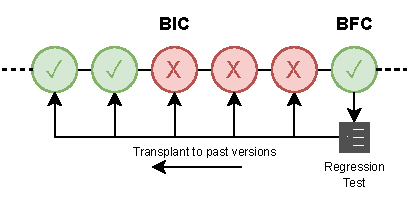
\includegraphics[width=0.8\textwidth]{pages/03-BugHunter/images/Model_Inverted.pdf}
  \vspace{-0.5cm}
  \caption{Simplified process leading to finding the first failing change (FFC), by running tests in past snapshots of the project.}
  \label{fig:process}
  \vspace{-0.5cm}
\end{figure}

The paper presenting the perfect test method~\cite{rodriguez2020bugs} states that one of the main limitations of the perfect test is that being able to construct a perfect test requires a deep knowledge of the bug, how it was fixed, and the project in which it was found. 
In our case, we assume that developers writing regression tests have all this knowledge, and therefore their tests will be close to the theoretical perfect test for the bugs they fix.


\subsection{The bugs dataset}
\label{subsec:dataset}

Defects4J~\cite{just2014defects4j} is a well-known dataset with 835 bugs from 17 Java open source software projects, including only bugs located in the source code, excluding those related to the build system, configuration files, documentation or tests. It has been used as ground truth in the evaluation of several implementations of SZZ-derived algorithms~\cite{neto2019revisiting,pokropinski2022szz,wen2019exploring,an2021reducing}. 
Previous studies have identified several issues that might threaten application of SZZ-derived algorithms: e.g., links to the repositories might have  changed~\cite{lawrence2001persistence}, repositories might have been deleted, moved, made private, or their history might have been altered~\cite{bird2009:promises_perils_git}.
However, Defects4J includes the whole source code management repositories of each project, avoiding the problems mentioned above.
All but one of the repositories in Defects4J are git repositories, which is the source code management we will target in our study.

% Defects4J is not only a dataset, but a whole framework for working with the repositories and bugs it includes. \as{This seems to contradict the first sentence of this section ``Defect4J is a well-known dataset...'' Please rephrase.}
% It provides a command-line tool for extracting information related to a bug (e.g., the fixing commit, the bug report, and the regression test), \as{This is odd: so far there has been no discussion that Defect4J contains fixing commits, this point will be made only in the next paragraph. Maybe move this paragraph further downwards?} get a copy of the corresponding repository, and other useful tasks, which makes it easy to work with the dataset. \as{The last fragment ``and other useful tasks...'' does not seem to be useful.}

Every bug included in Defects4J identifies the change (commit) fixing it (its BFC), and refers to a publicly available bug report which details the nature of the bug.
From here on we refer to changes as commits, since we will focus on git repositories.
% \as{It seems that we are using the words ``change'' and ``commit'' interchangeably. Moreover, we are also calling the same thing a ``node''. Can we maybe select one of the terms and use it consistently?}
% \michel{Now, from the second paragraph of Section~\ref{subsec:dataset} where the term commit is stated as the "change" defined above, only the term "commits" is used. The term "change" is kept in the Section~\ref{subsec:model} to be consistent with Gema's work.}
% \as{OK, we might like to add a sentence like ``From here on we refer to changes as commits'' or something similar.}
This bug report will be required when manually evaluating the detected BICs.
Therefore, the dataset complies with step (1) of the perfect test method. 
Associated with each bug there is also a regression test, included in the BFC, that exposes the bug. 
The dataset also provides its own commands to compile the code and execute the test in this commit. 
We will use this regression test as a perfect test for the bug, therefore complying with step (2) of the perfect test method.
Although the regression tests included in Defects4J have been reviewed by the authors of the dataset and emphasize in their tool that they have left out any flaky test, we have run each test 3 times in the BFC to verify that their results do not differ, and therefore we avoid including non-deterministic tests in the experiment.

The dataset does not include information about the commit that introduced the bug (if any), which we would need to verify that the result of step (3) of the perfect test method found the right change. 
However, the dataset provides a specific (synthetic) snapshot of the code without the fix (that is, with the bug present), in which we can check that the test fails. 
This supports our assumption that the regression tests identified in the Defects4J dataset can be used as perfect tests.

% \as{It seems that the previous paragraphs where describing the dataset as is, while the remaining part of the subsection discusses what we have done to it (excluding some parts). Would it be a good idea to split 3.2 into 3.2.1 and 3.2.2?}
% After examining the dataset, we found that the projects in it use different build systems, \as{At this point it is not clear why is it even important to know what build systems are used by the projects. Consider making this explicit.} among which we identified Maven, Gradle and Ant (all common Java build systems).\as{Is the comment ``all common Java build systems'' really necessary?}
%  In our case, we decided to build snapshots, and execute the transplanted tests, only with Maven or Ant. 
% Maven is one of the most widely used build systems in Java and offers the least problems when reproducing a build~\cite{sulir2016quantitative}. 
% Additionally, we also use Ant because many projects using Maven had used Ant at some moment in the past (Maven replaced Ant as the build system in many projects, including some in the dataset\as{Do we have a reference to support the claim that many projects moved from Ant to Maven?}). 
% Therefore, for transplanting tests to any commit in the past history of projects using Maven, in some of them we also need to support Ant. 
% Including Gradle didn't significantly increase our chances\as{I am not sure that the phrasing in terms of chances is precise; maybe rephrase?} of building snapshots and running tests, as only one of the projects selected uses Gradle, and this project also offers support for Ant, so it is included in our study.

From the whole Defects4J collection of projects, we excluded project Chart because it uses Subversion~\footnote{\url{https://subversion.apache.org/}} as version control system. 
We focus only on projects that use Git. 
As a result, we included in our experiment 16 projects out of the 17 found in Defects4J, with a total of 809 bugs of the initial 835 bugs.
Table~\ref{table:dataset-table} shows a brief description of the selected projects: the number of bugs it contains reported by the dataset, the number of stored commits, the dates for the first commit of the project and the last one (the last commit does not correspond to the last one in the official repository, since the projects in the dataset are stored as a copy of the git repository at a specific point in time). 
It should be noted that this dataset was extended in 2020, based on the original 2014 dataset~\cite{just2014defects4j}.

\begin{table}[]
    \caption{\label{table:dataset-table} Description of the projects used from Defects4J}
    \resizebox{\textwidth}{!}{%
        \begin{tabular}{|r|r|r|r|r|}
            \hline
            \textbf{Project} & \textbf{\# of bugs} & \textbf{\# of commits} & \textbf{First Commit} & \textbf{Last Commit} \\ \hline
            Cli              & 39                  & 914                    & 2002-06-10            & 2019-03-25           \\ \hline
            Closure          & 174                 & 2,898                   & 2009-11-03            & 2013-12-13           \\ \hline
            Codec            & 18                  & 1,795                   & 2003-04-25            & 2019-04-23           \\ \hline
            Collections      & 4                   & 3,091                   & 2001-04-14            & 2019-03-25           \\ \hline
            Compress         & 47                  & 2,682                   & 2003-11-23            & 2019-03-25           \\ \hline
            Csv              & 16                  & 1,290                   & 2005-12-17            & 2019-04-14           \\ \hline
            Gson             & 18                  & 1,476                   & 2008-09-01            & 2019-11-05           \\ \hline
            JacksonCore      & 26                  & 1,724                   & 2011-12-22            & 2019-04-24           \\ \hline
            JacksonDatabind  & 112                 & 5,241                   & 2011-12-22            & 2019-05-15           \\ \hline
            JacksonXml       & 6                   & 949                    & 2010-12-30            & 2019-05-05           \\ \hline
            Jsoup            & 93                  & 1,261                   & 2010-01-17            & 2019-07-04           \\ \hline
            JxPath           & 22                  & 598                    & 2001-08-23            & 2018-05-15           \\ \hline
            Lang             & 64                  & 3,596                   & 2002-07-19            & 2013-10-10           \\ \hline
            Math             & 106                 & 4,913                   & 2003-05-12            & 2013-10-16           \\ \hline
            Mockito          & 38                  & 3,262                   & 2007-11-15            & 2016-08-02           \\ \hline
            Time             & 26                  & 1,718                   & 2003-12-16            & 2013-12-04           \\ \hline
        \end{tabular}
    }
\end{table}

%Defects4J can be used to check if the operationalization of the perfect test method by using regression tests actually detects the commit that introduced each of the bugs. \as{It seems that the previous sentence is much more precise than the current phrasing of the RQ. Maybe rephrase the RQ?}
% For this, we check if step (3) of the method, which finds the FFC for the test, actually detects the BIC for the given bug.

\subsection{Transplanting the test to the past}
\label{subsec:transplant} 

Following the process shown in Figure~\ref{fig:process}, we have designed and implemented a Python tool that automates all the necessary tasks to transplant the regression test to the commits corresponding to past changes, and run it to determine if it fails or succeeds. 
For each bug in our subset of the dataset, it takes the following steps:

\begin{enumerate}
  \item \textbf{Extract information.} 
    By using the command-line tool provided by Defects4J, extract the fix commit, bug report and regression test for the bug.
  \item \textbf{Set up the repository.} 
    By using the Defects4J command-line tool, obtain a copy of the git repository of the project corresponding to the bug.
  \item \textbf{Execute the regression test on the fix commit.} 
    This will ensure that the test actually succeeds for this snapshot, which means that it succeeds when the bug is fixed (if not, the test would not check properly, as the perfect test method states). For this, the tool checkouts the snapshot corresponding to the bug fixing commit (BFC), and runs the regression test on it.
    In this step, the file containing the test is stored, in order to be transplanted into the previous snapshot (the test method, as well as the file name and the path where it is located is provided by the dataset).
  % \item \textbf{Execute the regression test in the commit prior to the fix.}
  %   This will ensure that the test actually fails in this snapshot, confirming that it detects the bug properly (if it succeeds, the test is not detecting the bug properly, in the sense defined by the perfect test method). 
  %   For this, checkout the snapshot corresponding to the previous commit, transplant the regression test, and try to run it.
  %   We refer to transplanting as placing the file containing the test (copied from the BFC) in the original path (recreating the original directory if necessary).
  \item \textbf{Execute regression test on all previous commits.}
    This will allow us to find the first failing change (FFC), which as we discussed, in the case of intrinsic bugs, will be the BIC that we are looking for. For this, the tool checkouts each of those past commits, transplants the test to each of them, and runs it in each of them. 
    The FFC will be the first one that fails after the last one that succeeds. 
    %The list of past commits is obtained through the command \textit{git log --reverse}, run from the BFC.
\end{enumerate}

In the steps that execute regression tests, the tool follows this procedure:
\begin{inparaenum}[\bf(1)]
\item \textit{checkout the corresponding commit},
\item \textit{transplant (copy) the regression test},
\item \textit{compile the source code},
\item \textit{compile the regression test}, and
\item \textit{execute the regression test}.
\end{inparaenum}
For compiling and executing we decided to use standard Maven and Ant commands, since the command provided by Defects4J only works with some specific commits (in the BFC and in a synthetic commit where the bug is present), and we needed to build and run the test on any of them (see previous discussion on finding the FFC at Section~\ref{subsec:model}). 
%However, we used the copy of external libraries provided with Defects4J, thus avoiding problems due to some of them no longer being available.

When the tool finishes all actions for a given bug, it reports the results of executing the regression test (if that was possible) for all commits prior to the BFC. These results include the success or failure of the different phases: building the source code, building the transplanted test code, running the regression test, and the result (fail or success) of running the test. 
In order to know the reasons for failures, the tool also keeps a log of the execution of each step.

In order to measure how far a test can be transplanted to the past and answering \textbf{RQ\textsubscript{3.1A}}, it is necessary to define a metric that allows us to measure how far we can transplant a regression test. 
We propose the \textit{Transplantability} metric. 
For a given bug for which we have a test that detects it, we consider all commits that are ancestors of the BFC, in chronological order, and from this ordering we will find a commit $n$ which is the oldest at which the test can be transplanted and executed. 
We define \textbf{Transplantability (in days)}, $T_{days}$ as the number of days between commit $n$ and the BFC. 
In the same way, we define \textbf{Transplantability (in commits)}, $T_{commmits}$ as the number of commits between 
%\as{What does ``between'' mean for a tree? Is there always a branch between $n$ and the BFC?}\michel{We consider the chronological order (as stated above), not the branches.} \as{Where did we say this? Do we want to somehow integrate this chronological idea in the definition of $T_{commmits}$? Is it not odd to somehow count commits belonging to completely different branches?}
%\michel{We rephrased the first part of the paragraph to explain that the commits are traversed in chronological order.}
commit $n$ and the BFC.
The two different ways of quantifying, together, are intended to give a more comprehensive view of how far we can transplant a test into past commits.

In Chapter~\ref{chapter:buildability} we had already stated that at least in the compilation of the source code we may face problems that will prevent us from continuing with the experiment. 
We also consider the likelihood that errors may also occur in the compilation of the regression test and in the execution of the test itself (i.e., that the test does not generate a report indicating whether the test passes or fails).

Problems related to compilability of source code, the compilability of the regression test code (the transplanted test), and the runnability of the regression test will be studied in order to answer \textbf{RQ\textsubscript{3.1B}}. 
To further understand these problems, we introduce three definitions: source code compilability, transplanted test compilability, and transplanted test runnability.

\textbf{Source code compilability} is defined as the percentage of snapshots in the past history of the BFC that could be successfully compiled.
This metric was originally defined by Tufano et al.~\cite{tufano2017there} and used in Chapters~\ref{chapter:buildability} and~\ref{chapter:testability}.
These previous studies took as reference commit the last one in the repository (the most recent one), considering as the commit history of the project all the commits previous to this one. 
In this chapter we will use as reference the BFC commit to define the commit history for each bug. In this way, we will calculate the Source code compilability of the commits previous to the BFC.

\textbf{Transplanted test compilability} is similar, but for the transplanted test: the percentage of snapshots in the past history of the BFC in which we could compile the transplanted test. 
These parameters let us know how often the reason for not being able of running the transplanted test was not being able to compile the test itself or compiling the source code in each of the snapshots.

\textbf{Transplanted test runnability} is defined as the percentage of snapshots in the past history of the BFC in which we could run (execute) the transplanted test without errors, producing a ``success'' or ``fail'' result, as stated in Chapter~\ref{chapter:testability}. The larger the test runnability, the more commits in which we could run the test. If it is 100\%, the perfect test method can be run for the whole history before the BFC. When test runnability is not 100\%, for some commits we cannot assess if the test fails or succeeds (because it doesn't run). Depending on success and fail in other commits, maybe we have to add the commit to the list of candidate BICs without being able of be more conclusive about it. Therefore, the transplanted test runnability shows how successful is the transplantation of regression tests to past commits.

\subsection{Identifying the Bug Introducing Change}
\label{subsec:identify-bic}

From the results obtained after transplanting the regression test on the commits prior to the BFC we can seek to locate the BIC.
At this point, we can revisit what ``all previous commits'' from Step 4 mean. 
In Figure~\ref{fig:process} we present the history of commits as linear. 
However, in a real git repository the commit history might not be linear: there are development models (as GitFlow~\footnote{\url{https://nvie.com/posts/a-successful-git-branching-model/}}) with git in which development is done in parallel branches, which are merged when convenient. 
Therefore, the history of a project can be considered as a directed graph. 
The previous theoretical model contemplated only a linear history of commits, which limits the understanding of this history. The consideration of the history as a graph to further refine the BIC search is a contribution of this work.
Each node represents a commit that will point to the commits that precede it (its parents), which can be one or more.

With this in mind, we developed Algorithm~\ref{alg:bic} to detect the BIC in this graph. 
This algorithm receives as parameters the graph, annotated with the result of running the tests (its status, which can be success, fail or error) and the identification of the BFC in that graph. 
%This algorithm returns the list of candidates to be the BIC. 
This algorithm traverses the graph using a depth-first search~\cite{cormen2022depthfirstsearch}, starting with an empty list of candidates, and trying to find the list of candidates to be the BIC, according to the perfect test method. 
For that, the algorithm finds the node $n$ in which the test fails and which preceding nodes succeed (success parents), which would make $n$ a candidate to be the BIC.

Since for some nodes we could not run the test (because it could not be compiled, it did not run, or the source code could not be compiled), we must consider that in these nodes the tests may or may not be executed successfully.
%Therefore, the algorithm finds all nodes in which the test fails, or cannot be run, and in all nodes preceding these nodes the test succeeds, or cannot be run. 
%All the nodes found by the algorithm would be the candidates to be the BIC.
\begin{footnotesize}
    \begin{algorithm}[t!]
        \caption{Algorithm to detect bug-inducing commits}\label{alg:bic}
        \SetKwInOut{Input}{Input}
        \SetKwInOut{Output}{Output}
        \SetKwInOut{Precondition}{Precondition~}
        \Input{A $\mbox{\sl graph}$ (commit history) and the $\mbox{\sl bfc}$}
        \Output{A list of candidates for BIC}
        \Precondition {The $bfc$ status (the output of the regression test) must be success
        % \as{I understand the intention but ``status'' does not seem to be defined. }
        % \michel{I clarify what ``status'' is at text}
        % \as{It might be a good idea to explain ``status'' here such that the algorithm becomes self-contained?}
        }

        $candidates \gets []$\;
        $queue \gets [bfc]$\;
        $visited \gets [bfc]$\;
        $temp\_candidates \gets []$\;
        
        \While{$ NotEmpty(queue) $}{
            $n \gets GetFirst(queue)$\;
            \If{hasFailStatus(n)}{
                $candidates \gets []$\;
            }
            $parents \gets GetParents(graph, n)$\;
            $successParents \gets True$\ \Comment*[r]{Control if all parents are success} 
            % \as{What does $successParents$ mean?}
            % \michel{I clarify at text}
            \If{$ isEmpty(parents) $\Comment*[r]{Reach first commit}}{
                    \eIf{size(queue) == 0}{
                        $break$\;
                    }{
                        $continue$\;
                    }
            }

            \For{$p \in parents$}{
                $successParents \gets successParents \And hasSuccessStatus(p)$\;
                \If{$ \neg hasSuccessStatus(p) $}{
                    \If{$ hasErrorStatus(p) $}{
                        $AddItem(candidates, n)$\;
                    }
                    \If{$ p \notin visited $}{
                        $AddItem(queue, p)$\;
                        $AddItem(visited, p)$\;
                    }
                }
            }
            \If{$ successParents \And \neg hasSuccessStatus(n) $}{
                \eIf(){$ hasFailStatus(n) $}{
                    \Return{$[n]$}\; 
                }{
                    $AddItem(candidates, n)$\;
                    
                    \eIf(){IsEmpty(queue)}{
                        \Return{$candidates$}\;
                    }{
                        $temp\_candidates \gets candidates$\;
                    }
                    
                }
            }
        }
        \Return{$temp\_candidates$} 
    \end{algorithm}
\end{footnotesize}

The algorithm operates under the following assumptions: (1) all the ancestors of the BIC are success commits, until the beginning of the history of the project, or until the features on which the test is built are introduced; (2) in the case of a commit with two or more parents, which generate branches, the BIC can only be in one of these branches.
The first assumption is based on the definition of the BIC: the first commit where the bug manifests, which following the perfect test method, means the first commit where the test fails. In other words, in snapshots previous to the BIC the bug is not present, and therefore the test, if it can be run, should succeed. The test may not run if it is designed on top of some feature (e.g., some function) that does not exist for some snapshot, because it was not yet implemented.
The second assumption is based on the unlikeness that the same bug (which is fixed by a single fix commit) is introduced in two different branches. 
% For any given bug, it may happen that the test does not succeed in the BFC. 
% This may happen because the source code or the test is not compilable, in which case we can say nothing: we just do not have enough evidence to guarantee that the test actually succeeds for the BFC, and therefore we do not run it (we considered this as a precondition for identifying the BIC). We will consider that we do not have enough data for this bug, and will ignore it in our study.

Our algorithm has as a precondition that the regression test can be run and gives a successful result in the BFC.
If this precondition is fulfilled, we can run the algorithm, and come with two different outcomes:

\begin{itemize}
\item \textbf{The test succeeds in some preceding commit.}
  We should find at least one parent commit of the BFC for which the test fails (we should have at least one snapshot where the bug is present). 
  Following the ancestors of those commit that fail, we eventually find one that succeeds. 
  If we find a commit $n$ where the test does not succeed, but it succeeds for all its parents, then $n$ should be considered the commit that introduced the bug. 
  In this case, the algorithm found a single candidate and returns it. If we find a commit $n$ where the test cannot be compiled, and it succeeds in all its parents, then all commits between $n$ and $m$, being $m$ the first descendant of $n$ where the test can be compiled and fails, are considered candidates. 
  In this case, we have found several candidates, and we cannot decide which one is exactly the BIC because we cannot run the test in them, but we know the BIC should be one of them.
\item \textbf{The test does not succeed in any precedent commit.}
  In this case, we should assume that the bug was always in the code, since the functionality tested by the test was introduced or that we cannot run the test for some reason (i.e., we are not able to compile the source code). In any case, we cannot find the BIC: either it doesn't exist, or it is hidden because we cannot run the test, so the algorithm returns an empty list of candidates.
\end{itemize}

As an example of how the algorithm works, Figure~\ref{fig:bug41} represents the commit history for Bug 41 of the JacksonDatabind project from Defects4J dataset. 
The figure includes only commits relevant to understanding how the algorithm finds the BIC, and consecutive commits (without forks or merges) of the same color have been reduced to one. 
Each commit is identified with a number, whose value simply indicates its chronological position with respect to the fix commit (BFC) in order to be able to refer to them.
Colors in the figure show if the regression test succeeds (green~\checkmark) or fails (red~$X$).

\begin{figure}[ht!]
  \centering   
  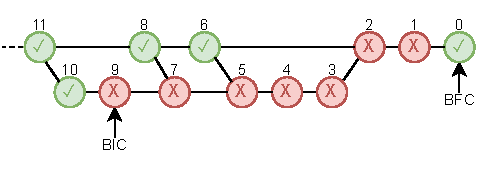
\includegraphics[width=\columnwidth]{pages/03-BugHunter/images/Databind_41_Inverted.pdf}
  \caption{Visual representation of the results of the experiment for Bug 41 of JacksonDatabind project.}
  \label{fig:bug41}
\end{figure}

In this figure we can see how Commit 2, although it has a green parent (Commit 6), cannot be considered as BIC, since it has another parent (Commit 3) where the bug is present. Following the ancestors chain, the algorithm will at some point find Commit 9, which is red, but for which all parents are green (in this case, only Commit 10). 
%All ancestors of Commit 10 are green too. 
Therefore, the candidate list in this case will include only Commit 9.

% As stated before, all the is fully automated in a tool implemented as a set of Python scripts (see Figure~\ref{fig:tool}). First, information about the bug (the BFC, the regression test that reveals the bug and the link to the test report) and the corresponding Git repository are extracted by \textit{ExtractBugsD4J.py} using the command-line tool provided by Defects4J (D4J). Then, the regression test is run on the BFC and all the commits preceding it, using \textit{RegTestExecutor.py}. The results of the building process for each commit, and the result of running the test is recorded. \textit{CommitGraph.py} uses these results to produce a labeled graph (with labels showing the results of building and test running), which is fed to \textit{Analysis.py}, which runs the Algorithm~\ref{alg:bic} to find BIC candidates.

% \begin{figure}[t!]
%     \centering   
%     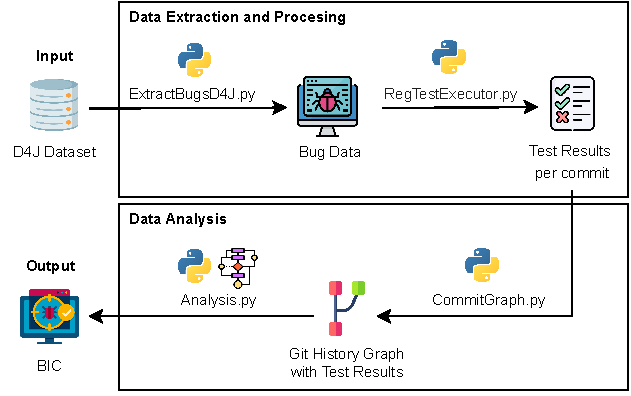
\includegraphics[width=\columnwidth]{images/RegressionTool.pdf}
%     \caption{Processes carried out by the tool. All scripts and documentation for the tool are available in the reproduction package (See `Reproducibility' section at the end of the paper).}
%     \label{fig:tool}
%     \vspace{-0.5cm}
% \end{figure}

%\as{This section seems to be too lengthy...}
%\michel{Huge refactor has been performed}

\subsection{Manual validation}
\label{subsec:manual}

To ensure that the results of our study can be considered as ground truth, we verified them by performing a manual validation of the BICs detected for each analyzed bug. For this purpose, we performed the following steps for each BIC detected:

\begin{itemize}
    \item Check and understand the bug report
    \item Check and understand the fixed functionality in the BFC.
    \item Check and understand the changed functionality in the candidate BIC
    \item Check the output of the test run
\end{itemize}

Following these steps, we categorized the BICs found in our study as true positives or false positives, using only true positives as the ground truth in order to generate a validated dataset of BICs.

%%% Local Variables:
%%% mode: latex
%%% TeX-master: "../paper"
%%% End:


\section{Experimental Results}
\label{sec:bug-hunter:results}
% jgb: Proposal for the text above
In this section we show the results of our study, answering the research questions presented in the introduction. 
The following results are intended to determine the extent to which we can operationalize the theoretical model proposed by \gema~
We have considered a total of 809 bugs in the Defects4J dataset, after filtering out bugs for the project we do not consider as explained in Section~\ref{subsec:dataset}. The results we found for each of those bugs are summarized in Figure~\ref{fig:experiment-overview}. 
This figure differentiates the cases in which, out of the total number of bugs, the regression test was found to pass again in some commit prior to the BFC from those that did not. In turn, from this first group, we differentiate the bugs from which we have been able to obtain a single candidate to be the BIC or several of them.
%\as{I guess that this figure should be somehow discussed?}
%\michel{I add a little explanation}

\begin{figure}[h!]
    \centering    
    % \begin{tikzpicture}[node distance=1cm,every node/.style={fill=white, font=\sffamily}, align=center]
%     % Specification of nodes (position, etc.)
%     \node (total)             [large]                                         { };
%     \node (buildable)         [large, below of=total]                         { };
%     \node (testBuildable)     [large, below of=buildable]                     { };
%     \node (success)           [large, below of=testBuildable]                 { };

%     \draw[-Latex]             (total) -- (buildable);
%     \draw[-Latex]             (buildable) -- (testBuildable);
%     \draw[-Latex]             (testBuildable) -- (success);

% \end{tikzpicture}
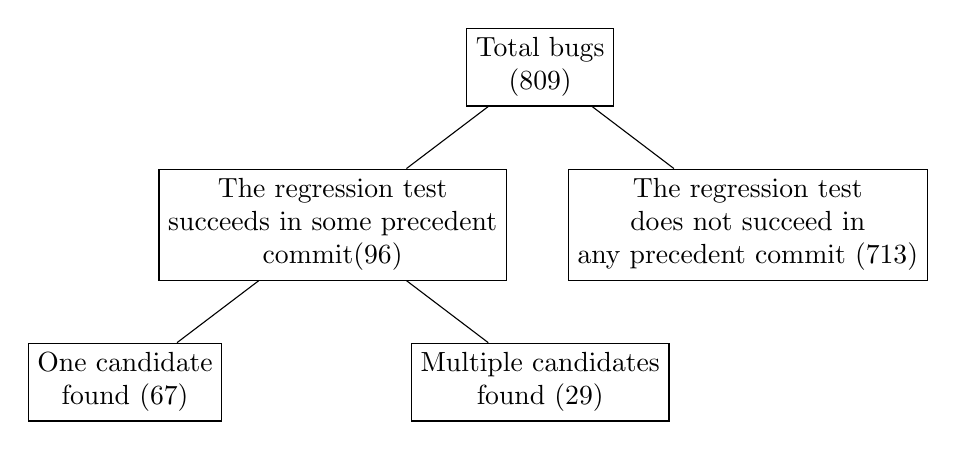
\begin{tikzpicture}[sibling distance=15em, level distance=2cm,
    every node/.style = {shape=rectangle, draw, align=center, top color=white,  }]
    \node {Total bugs \\ (809)}
      child { node {The regression test \\ succeeds in some precedent\\ commit(96)} 
          child { node {One candidate\\ found (67)} }
          child { node {Multiple candidates\\ found (29)} }
      }
      child { node {The regression test\\ does not succeed in\\  any precedent commit (713)} }
      ;
\end{tikzpicture}
  %  \vspace{-0.5cm}
    \caption{Summary of results for each of the bugs considered in the study.}
    \label{fig:experiment-overview}
\end{figure}

%%%%%%%%%%%%%
%    RQ1A    %
%%%%%%%%%%%%%

\subsection{How far can a test be transplanted into the past?}
\label{results:rq1a}

In Table~\ref{table:rq1a} we show the values for each of the interpretations of Transplantability for each bug. 
The values are aggregated by project, showing the mean and median for all bugs in each project. 
%The table also provides the aggregation of all bugs from all projects to obtain the mean and median Transplantability values for the dataset.
Additionally, we add in the table the relative position (\%) of commit $n$ (1) with respect to the total number of days elapsed between the BFC and the first commit of the project and (2) with respect to the total number of commits between the BFC and the first commit of the project. 
A value close to 0\% in this relative position indicates that we have barely been able to transplant the regression test, while values close to 100\% indicate that the test has been transplanted in most of the past (with respect to the BFC).

\begin{table*}[ht!]
    \caption{\label{table:rq1a} Transplantability (in days and in number of commits) for each bug, aggregated by mean ({\large $\mean{x}$}), 
    by median ({\large $\median{x}$}) and by the relative position of the oldest commit where the test could be transplanted ({$\%$}).}
    \resizebox{\textwidth}{!}{%
        \begin{tabular}{|r|r|rrr|rrr|}
            \hline
            \multicolumn{1}{|c|}{}                 &                  & \multicolumn{3}{c|}{$T_{days}$}                                                   & \multicolumn{3}{c|}{$T_{commmits}$}\\
            %\cline{3-8} \\
            \multicolumn{1}{|c|}{\textbf{Project}} & \textbf{\# bugs} & \multicolumn{1}{c|}{\textbf{\large{\large $\mean{x}$}}} & \multicolumn{1}{c|}{\textbf{\large{\large $\median{x}$}}} & \multicolumn{1}{c|}{\textbf{\%}} & \multicolumn{1}{c|}{\textbf{\large{\large $\mean{x}$}}} & \multicolumn{1}{c|}{\textbf{\large{\large $\median{x}$}}} & \multicolumn{1}{c|}{\textbf{\%}} \\ \hline
            \textbf{Cli}                            & 39                                     & \multicolumn{1}{r|}{910}  & \multicolumn{1}{r|}{1168} & 36.09                 & \multicolumn{1}{r|}{134}  & \multicolumn{1}{r|}{115}  & 34.67                 \\ \hline
            \textbf{Closure}                        & 174                                    & \multicolumn{1}{r|}{234}  & \multicolumn{1}{r|}{108}  & 36.63                 & \multicolumn{1}{r|}{451}  & \multicolumn{1}{r|}{187}  & 39.62                 \\ \hline
            \textbf{Codec}                          & 18                                     & \multicolumn{1}{r|}{703}  & \multicolumn{1}{r|}{427}  & 27.06                 & \multicolumn{1}{r|}{192}  & \multicolumn{1}{r|}{78}   & 26.12                 \\ \hline
            \textbf{Collections}                    & 4                                      & \multicolumn{1}{r|}{599}  & \multicolumn{1}{r|}{703}  & 11.05                 & \multicolumn{1}{r|}{178}  & \multicolumn{1}{r|}{213}  & 6.30                  \\ \hline
            \textbf{Compress}                       & 47                                     & \multicolumn{1}{r|}{1885} & \multicolumn{1}{r|}{2021} & 47.64                 & \multicolumn{1}{r|}{1223} & \multicolumn{1}{r|}{1326} & 82.18                 \\ \hline
            \textbf{Csv}                            & 16                                     & \multicolumn{1}{r|}{106}  & \multicolumn{1}{r|}{41}   & 3.11                  & \multicolumn{1}{r|}{41}   & \multicolumn{1}{r|}{27}   & 5.17                  \\ \hline
            \textbf{Gson}                           & 18                                     & \multicolumn{1}{r|}{1283} & \multicolumn{1}{r|}{1212} & 47.60                 & \multicolumn{1}{r|}{481}  & \multicolumn{1}{r|}{368}  & 41.70                 \\ \hline
            \textbf{JacksonCore}                    & 26                                     & \multicolumn{1}{r|}{444}  & \multicolumn{1}{r|}{450}  & 32.98                 & \multicolumn{1}{r|}{262}  & \multicolumn{1}{r|}{258}  & 34.00                 \\ \hline
            \textbf{JacksonDatabind}                & 112                                    & \multicolumn{1}{r|}{718}  & \multicolumn{1}{r|}{666}  & 43.92                 & \multicolumn{1}{r|}{1183} & \multicolumn{1}{r|}{1123} & 40.74                 \\ \hline
            \textbf{JacksonXml}                     & 6                                      & \multicolumn{1}{r|}{884}  & \multicolumn{1}{r|}{939}  & 40.49                 & \multicolumn{1}{r|}{256}  & \multicolumn{1}{r|}{239}  & 40.41                 \\ \hline
            \textbf{Jsoup}                          & 93                                     & \multicolumn{1}{r|}{437}  & \multicolumn{1}{r|}{240}  & 26.95                 & \multicolumn{1}{r|}{142}  & \multicolumn{1}{r|}{76}   & 18.33                 \\ \hline
            \textbf{JxPath}                         & 22                                     & \multicolumn{1}{r|}{607}  & \multicolumn{1}{r|}{532}  & 24.44                 & \multicolumn{1}{r|}{80}   & \multicolumn{1}{r|}{79}   & 21.65                 \\ \hline
            \textbf{Lang}                           & 64                                     & \multicolumn{1}{r|}{355}  & \multicolumn{1}{r|}{246}  & 14.88                 & \multicolumn{1}{r|}{283}  & \multicolumn{1}{r|}{206}  & 13.05                 \\ \hline
            \textbf{Math}                           & 106                                    & \multicolumn{1}{r|}{186}  & \multicolumn{1}{r|}{110}  & 7.60                  & \multicolumn{1}{r|}{280}  & \multicolumn{1}{r|}{178}  & 10.16                 \\ \hline
            \textbf{Mockito}                        & 38                                     & \multicolumn{1}{r|}{1664} & \multicolumn{1}{r|}{1552} & 96.61                 & \multicolumn{1}{r|}{1781} & \multicolumn{1}{r|}{1540} & 95.93                 \\ \hline
            \textbf{Time}                           & 26                                     & \multicolumn{1}{r|}{452}  & \multicolumn{1}{r|}{478}  & 28.02                 & \multicolumn{1}{r|}{97}   & \multicolumn{1}{r|}{77}   & 19.33                 \\ \hline
            \hline
            \textbf{All bugs}                       & 809                                    & \multicolumn{1}{r|}{585}  & \multicolumn{1}{r|}{302}  & 32.93                 & \multicolumn{1}{r|}{530}  & \multicolumn{1}{r|}{212}  & 33.83                 \\ \hline
        \end{tabular}
    }
\end{table*}


For a more comprehensive view of the Transplantability results, Table~\ref{table:rq1a-iqr} provides in detail the distribution of $T_{days}$ and $T_{commits}$ results.
First, we found that both metrics offer very similar results, showing that the average frequency with which a commit is added to these repositories is approximately 1 day. 
% \michel{Here I think a reviewer could tell us why we use two metrics that mean the same thing. Although it may seem intuitive, I have read other articles about the frequency of commits per day in open source projects and they are around 4 commits/day on average.}\as{I think that this was some of Gregorio's work? We need to comment on this.}
Regarding the minimum value for both metrics, we found the value 0, which indicates that for at least one project, it was not possible to transplant the test to the commit prior to the BFC. We found that for bug 79 of the Closure project the BFC includes a new function as part of the bug fix, being this function used in the regression test. Since this function does not exist in the previous commits to the BFC, the error obtained when transplanting the test to them is a failure in the compilation of the test code.

\begin{table*}[]
    \caption{\label{table:rq1a-iqr} Distribution of Transplantability results for all projects}
    \resizebox{\textwidth}{!} & \textbf{50\%} & \textbf{75\%} & \textbf{max} \\ \hline
      \textbf{$T_{days}$}    & 809              & 585           & 706          & 0            & 84            & 302           & 830           & 3,475         \\ \hline
      \textbf{$T_{commits}$} & 809              & 530           & 696          & 0            & 72            & 212           & 712           & 3,709         \\ \hline
      \end{tabular}
    }
\end{table*}

In order to evaluate the feasibility of our method, we check whether the BIC found by our tool falls within the $T_{commits}$ and $T_{days}$ for the different regression tests. In this case we can assume that, at least for the considered projects, the test can be transplanted far enough to allow the detection of the BIC. 
For the 67 BICs detected, we found that, on mean, they are 182 days  and 190 commits between the BIC and the BFC. 
The diversity of projects forces us to check, in addition, the median: 47 days and 49 commits respectively. 
According to the values of $T_{days}$ and $T_{commits}$ we can state that we have been able to transplant the regression tests far enough to be useful in detecting the BIC. 
%\as{This is an extremely bold statement. To claim usefulness we need to somehow hear this from the developers of the original projects but this is probably impossible since the data is likely to be old. Is there a way to say something about ``far enough'' without asking developers?}
%\michel{We rephrased the statement to focus on the ``feasibility'' of the method}

Nevertheless, there might be commits between $n$ and the BFC where the regression test cannot be compiled or run. This leads us to the next RQ.

\vspace{0.4cm}
\fbox{\begin{minipage}{0.9\textwidth}
    \textbf{\rqonea}
    For the dataset used, we have managed to transplant the regression test for a bug up to 585 days (530 commits) in the past on average. 
    For 50\% of the bugs, the regression test could be transplanted up to at least 302 days (212 commits).
    On average, regression tests can be transplanted to a 32.93\% of the days (33.83\% of the commits) between the BFC and the initial commit of the project.
\end{minipage}}

%%%%%%%%%%%%%
%    RQ1B    %
%%%%%%%%%%%%%

\subsection{How compilability and runnability problems impact the transplantation of the regression tests to the past?}
\label{results:rq1b}

In Table~\ref{table:results-per-project} we show average and mean data for the three metrics defined in Section~\ref{sec:bug-hunter:methodology}: source compilability, transplanted test compilability and transplanted test runnability.

\begin{table}[h!]
    \centering{\small
        \caption{\label{table:results-per-project} Source code compilability, transplanted test compilability, and transplanted test runnability for each bug, aggregated by mean ({\large $\mean{x}$}) and by median ({\large $\median{x}$}) per project. 
        Values are shown in percentages.}
        \begin{tabular}{|r|r|rr|rr|rr|}
            \hline
            \multicolumn{1}{|c|}{\multirow{2}{*}{\textbf{Project}}} & \multicolumn{1}{c|}{\multirow{2}{*}{\textbf{\# bugs}}} & \multicolumn{2}{c|}{\textbf{\begin{tabular}[c]{@{}c@{}}Source \\ Compilability\end{tabular}}} & \multicolumn{2}{c|}{\textbf{\begin{tabular}[c]{@{}c@{}}T.Test \\ Compilability\end{tabular}}} & \multicolumn{2}{c|}{\textbf{\begin{tabular}[c]{@{}c@{}}T.Test \\ Runnability\end{tabular}}} \\ %\cline{3-8} 
            \multicolumn{1}{|c|}{}                                  & \multicolumn{1}{c|}{}                                     & \multicolumn{1}{c|}{\textbf{\large{\large $\mean{x}$}}}     & \multicolumn{1}{c|}{\textbf{{\large $\median{x}$}}}    & \multicolumn{1}{c|}{\textbf{{\large $\mean{x}$}}}    & \multicolumn{1}{c|}{\textbf{{\large $\median{x}$}}}   & \multicolumn{1}{c|}{\textbf{{\large $\mean{x}$}}}   & \multicolumn{1}{c|}{\textbf{{\large $\median{x}$}}}   \\ \hline
            \textbf{Cli}                            & 39                                     & \multicolumn{1}{r|}{56.07} & 62.61                 & \multicolumn{1}{r|}{29.40} & 30.88                 & \multicolumn{1}{r|}{29.40} & 30.88                 \\ \hline
            \textbf{Closure}                        & 174                                    & \multicolumn{1}{r|}{59.24} & 54.36                 & \multicolumn{1}{r|}{33.52} & 17.63                 & \multicolumn{1}{r|}{33.52} & 17.63                 \\ \hline
            \textbf{Codec}                          & 18                                     & \multicolumn{1}{r|}{28.30} & 14.29                 & \multicolumn{1}{r|}{25.13} & 8.84                  & \multicolumn{1}{r|}{25.13} & 8.84                  \\ \hline
            \textbf{Collections}                    & 4                                      & \multicolumn{1}{r|}{97.94} & 98.98                 & \multicolumn{1}{r|}{5.73}  & 7.46                  & \multicolumn{1}{r|}{5.61}  & 7.37                  \\ \hline
            \textbf{Compress}                       & 47                                     & \multicolumn{1}{r|}{29.96} & 23.60                 & \multicolumn{1}{r|}{20.81} & 17.02                 & \multicolumn{1}{r|}{18.35} & 10.22                 \\ \hline
            \textbf{Csv}                            & 16                                     & \multicolumn{1}{r|}{19.07} & 17.38                 & \multicolumn{1}{r|}{5.26}  & 3.51                  & \multicolumn{1}{r|}{5.21}  & 3.51                  \\ \hline
            \textbf{Gson}                           & 18                                     & \multicolumn{1}{r|}{42.00} & 35.98                 & \multicolumn{1}{r|}{40.73} & 34.68                 & \multicolumn{1}{r|}{40.73} & 34.68                 \\ \hline
            \textbf{JacksonCore}                    & 26                                     & \multicolumn{1}{r|}{35.08} & 32.54                 & \multicolumn{1}{r|}{31.52} & 30.12                 & \multicolumn{1}{r|}{31.52} & 30.12                 \\ \hline
            \textbf{JacksonDatabind}                & 112                                    & \multicolumn{1}{r|}{88.37} & 90.17                 & \multicolumn{1}{r|}{13.77} & 14.22                 & \multicolumn{1}{r|}{13.77} & 14.22                 \\ \hline
            \textbf{JacksonXml}                     & 6                                      & \multicolumn{1}{r|}{89.65} & 88.81                 & \multicolumn{1}{r|}{24.49} & 24.59                 & \multicolumn{1}{r|}{24.49} & 24.59                 \\ \hline
            \textbf{Jsoup}                          & 93                                     & \multicolumn{1}{r|}{21.08} & 12.52                 & \multicolumn{1}{r|}{17.56} & 9.74                  & \multicolumn{1}{r|}{17.56} & 9.74                  \\ \hline
            \textbf{JxPath}                         & 22                                     & \multicolumn{1}{r|}{92.25} & 100.00                & \multicolumn{1}{r|}{21.93} & 23.57                 & \multicolumn{1}{r|}{21.93} & 23.57                 \\ \hline
            \textbf{Lang}                           & 64                                     & \multicolumn{1}{r|}{74.08} & 66.08                 & \multicolumn{1}{r|}{11.61} & 8.50                  & \multicolumn{1}{r|}{11.61} & 8.50                  \\ \hline
            \textbf{Math}                           & 106                                    & \multicolumn{1}{r|}{39.80} & 36.19                 & \multicolumn{1}{r|}{7.99}  & 5.86                  & \multicolumn{1}{r|}{7.99}  & 5.86                  \\ \hline
            \textbf{Mockito}                        & 38                                     & \multicolumn{1}{r|}{30.69} & 30.06                 & \multicolumn{1}{r|}{24.17} & 25.22                 & \multicolumn{1}{r|}{24.17} & 25.22                 \\ \hline
            \textbf{Time}                           & 26                                     & \multicolumn{1}{r|}{72.84} & 100.00                & \multicolumn{1}{r|}{20.72} & 6.47                  & \multicolumn{1}{r|}{18.89} & 4.12                  \\ \hline
            \hline
            \textbf{All}                            & 809                                    & \multicolumn{1}{r|}{53.43} & 49.89                 & \multicolumn{1}{r|}{20.92} & 12.36                 & \multicolumn{1}{r|}{20.71} & 12.00                 \\ \hline
        \end{tabular}
    }
    \vspace{-4mm}
\end{table}


Table~\ref{table:rq1b-iqr} provides in detail the distribution these metrics for a more comprehensive view of the results. 

\begin{table}[]
  \caption{\label{table:rq1b-iqr} Distribution of source compilability, transplanted test compilability and transplanted test runnability results for all projects}
  \resizebox{\textwidth}{!} & \textbf{50\%} & \textbf{75\%} & \textbf{max} \\ \hline
      \textbf{Src compilability}      & 809              & 53.43         & 32.26        & 0.26         & 24.88         & 49.89         & 84.45         & 100.0        \\ \hline
      \textbf{T.Test compilability}   & 809              & 20.92         & 23.93        & 0.10         & 4.26          & 12.36         & 26.67         & 100.0        \\ \hline
      \textbf{T.Test runnability}     & 809              & 20.71         & 23.98        & 0.10         & 4.12          & 12.00         & 26.58         & 100.0        \\ \hline
    \end{tabular}
  }
\end{table}

The reasons that prevent transplanting the regression test are directly related to these metrics and can be classified as follows:

\begin{itemize}
\item \textbf{Compilability of the source code} If the source code cannot be built for the snapshot, there is no way to build the regression test. 
Compilability of past snapshots has been studied in detail by Tufano et al.~\cite{tufano2017there},whose experiment in 2014 showed an average compilability of 100 Java projects of 37.74\%. 
As seen in Chapter~\ref{chapter:buildability}, we replicated this experiment in 2020 and a decrease in compilability was observed due to the lapse of time, 
%\as{Please be more explicit why the lapse of time could be expected to reduce the compilability value.} \michel{Below it is commented that one of the factors affecting compilability is the passage of time. I clarify it} 
obtaining a value of 25.09\%. The compilability may vary largely from project to project, and it will depend among other factors on the availability of third party modules needed to build the code, on the availability of the building tools in the right version, and on the complete automation of the building process. These factors are usually affected by time, and a degradation of compilability as time passes has been observed in these two previous studies.
In our case, the mean compilability of the snapshots previous of each bug is 53.43\% (with a median of 49.89\%). 
The value obtained is higher than that obtained in previous studies due to a combination of good practices by the authors of the Defects4J dataset; \patxi{Esto deberían ser dos puntos?}
% \as{do you mean that storing dependencies and adding configuration files are the good practices? Or are there some good practices (whatever they might be) and on top of them the developers store dependencies and adapt configuration files?}
% \michel{The configuration files and the storage of the libraries are the best practices that I want to emphasize. Further on I comment that it provides a high reproducibility of the experiments (understanding that these are good practices to follow for anyone who wants to make his dataset reproducible).} 
storing project dependencies and adapting their configuration files to ensure high reproducibility in the experiments (although only in the BFCs), together with additional adaptations made by the authors of this work, completing the adaptation of the configuration of each project to each commit of its history.
%\as{"relatively low" suggests comparison with some kind of baseline. How do our figures compare to those reported in the previous papers [36,22]?}
%\michel{Now is more clear and we have added the comparison with the previous studies + the reason why our results are higher + explain the modifications to improve the compilability.}
\item \textbf{Compilability of the regression test} If the test cannot be built, it cannot be run. The test is built on top of the snapshot, and it may not build because the code it expects in the snapshot is not present. This may happen because that code was still not implemented for a given snapshot. For example, this is the case if the test tests a certain function: in some past snapshot the function may not be implemented yet. This may also happen because the code was in the snapshot, but not in the way the test expects it. For example, this may happen in case of refactoring between the snapshot we are trying to build and the snapshot for which the test was designed. In general, these problems will be increasingly frequent for older commits with respect to the BFC, since more artifacts (code files, libraries or configuration files) could change since those snapshots to the one corresponding to the BFC, for which the regression test was designed. They will also be frequent in branches which for some reason lack some code needed by the test.
The aggregate results for the transplanted test compilability (20.92\% mean and 12.36\% median for all bugs) are strictly lower than source code compilability, since compiling the source code is a necessary step to be able to compile and run the tests. \patxi{This is different to the results from Chapther 4, where in general whenever the source code compiles, the tests compile as well. In this case, the fact that we are transplanting the test from the present to the past has an impact on its compilability.}
To the best of our knowledge, there is no large-scale study on the compilability of a test that is transplanted to past commits, so we do not have a baseline on which to compare the results obtained on this metric.
% \as{Can we find some kind of baseline to compare these numbers, similarly to the compilability figures for the source code?}
% \michel{There are no previous studies that transplant tests into the past and measure how far they can be taken. The closest is a study of ours (not yet published) in which we ran tests on all commits of a project.}
% \as{Can we comment that there is no publicly available baseline?}

\item \textbf{Runnability of the regression test} Even if the regression test can be built, maybe its run does not produce a result, but fails earlier due to some code not behaving as expected. 
% This may happen, for example, if the test calls some function that is expected to return a certain value, but returns some other because that was the case in the earlier version of the code corresponding to the snapshot. 
When aggregating all bugs together, the mean for transplanted test runnability is 20.71\%, and the median is 12\%. 
Which means that in half of the bugs the test could be transplanted successfully to less than 12\% of the commits (although the difference with the mean shows how in some bugs, the transplant was successful in a much higher fraction of the cases). 
These values are again slightly lower than the previous metric (the compilability of the regression test) since we need to compile the test code in order to be able to run it. In this case, the values are very close (or even equal) to those of the compilability of the regression tests, so we can affirm that if the transplanted test is successfully compiled, it can be executed.
Again, as far as we know, the runnability of a test transplanted to the past has not been addressed on a large scale.
Again, to the best of our knowledge, the runability of a test transplanted to the past has not been previously addressed.\patxi{La frase se repite dos veces?}
% \as{Also here, no other baselines?}
% \michel{Like the previous one, we have no previous study to compare ourselves with.}
% \as{As above?}
% In some projects, transplanting bugs to past commits usually works, with medians as high as 98.07\% in Gson, meaning that in this case for half the bugs tests could be transplanted to almost all commits. But in others, it rarely works, such as in Collections or Csv, where in half the bugs the test could be transplanted to less than 4\% of the commits.
\end{itemize}

We will discuss the problems of transplanting the tests in the past in more detail in Section~\ref{sec:transplant-discuss}.
% \michel{Initially, the (specific) problems why I could not transplant the test to the past belonged to the discussion. In this section we start from metrics (src/test compilability and runnability) and delve (not too much) into the reasons why they do not obtain higher values. In the specified section I describe in more detail which problems I found and how I solved them.}

When examining the numbers for each project, we can see how, even when it varies from project to project, transplanted test runnability is always very similar to transplanted test compilability, which means that if the test compiled, in general it runs. In other words: the main blocker for running a test is that the test does not compile. For compiling the test, we should compile the source code. Again, by looking at this table, we can see how in some cases, the blocker for compiling the transplanted test is that the snapshot does not compile (for example for Gson, in almost all commits for which the snapshot compiled, the test also compiled). But for most of them, even if the snapshot compiles, the test does not.

These results are relevant because they show that by improving the compilability of the source code, and of the regression test, we could improve transplanted test runnability, and therefore, the applicability of the perfect test method. They also show that some projects have a very low compilability. 
This may be due to age (See Table~\ref{table:dataset-table})
%\as{Maybe we need to describe each and every bug? In any case here we should refer to such a table/description...}
of those projects (maybe the developers of those projects were using old practices that do not interact well with modern tools), or to specific characteristics of those projects, that maybe could be fixed with more knowledge about their building configuration.

Despite all these factors, the fact that for some projects transplanted test runnability is high shows that at least in some cases the conditions to use the perfect test method with regression tests hold.

\vspace{0.4cm}
\fbox{\begin{minipage}{0.9\textwidth}
    \textbf{\rqoneb}
    The effectiveness of the transplant \patxi{transplantation?} is limited by compilability issues unrelated to the transplanted test (the snapshot does not compile 
    46.57\% of the time) or by compilability of the transplanted test (the test does not compile 79.08\% of the time, essentially because of the limitation in compiling the source code or because it relies on missing code). However, we found that when the test compiles, in general, the test can be run. Therefore, compilability of the source code is a blocker that, when improved, could improve the transplanted test runnability.
\end{minipage}}

%%%%%%%%%%%%%
%    RQ2    %
%%%%%%%%%%%%%

\subsection{Can the BIC for a given bug be found using its regression test?}
\label{sec:rq2}

Following on with the chart in Figure~\ref{fig:experiment-overview}, to answer $RQ_{3.2}$ we will study in which cases the test succeeded in some precedent commit, and in those cases, how many candidate BICs were found. We consider the following scenarios as defined in our methodology. 

\textbf{The test does not succeed in any previous commit.}

From the total 809 bugs, in 713 the regression test did not succeed in any commit previous to it. 
In these cases, the perfect test method (using regression test as perfect tests) does not allow us to identify candidates for being the BIC. 
Since the test never succeeds in commits previous to the BFC, we cannot find the commit in which the bug was introduced. 
In the snapshots corresponding to some of those commits this is because the test cannot be run (and therefore we don't know if the bug is present or not in them), and in some others because it can be run, but fails (and then we know that the bug is present).

The reasons for the test not running (the test was not successfully transplanted) were already explored in the previous section, and in many cases are related to compilability problems. 
The fact that the tests are executed (successfully transplanted) but fail in all commits prior to the BFC is a case contemplated and addressed by the perfect testing \patxi{test} method: it means that the bug is present in those snapshots since the feature tested was introduced.
However, if we cannot find a previous commit for which the test succeeds, we have no evidence of where the BIC is.

\textbf{The test succeeds again in some past commit.}

For the remaining 96 bugs, the test succeeds in at least one commit previous to the BFC, and therefore we can provide more conclusive results by running the perfect test method.

For 67 bugs out of these 96, our algorithm produces a single candidate to be the BIC. 
The regression test succeeds in snapshots previous to this BIC candidate, which means it is the FFC (First-Failing Change), and following the perfect test method, the commit that introduce the bug (BIC). 
In 8 of these cases, the BIC was found in a direct parent of the BFC, which means the bug was detected and fixed very quickly after it was introduced. 
This is due to a practice known as \textit{Backtracking}~\cite{yoon2012exploratory,yoon2014longitudinal}, where the developer reverts part or all of the change \patxi{changes?} made when an issue is reported.

For the 29 remaining bugs, the algorithm finds multiple candidates. 
If $n$ is the first commit (going backwards from the BFC) in which the test succeeds, we have several candidates if for one or more commits that are right before $n$ (again, going backwards from the BFC) the test could not be executed (we are not able to compile the code or the test).
In those cases, since the test could not be run, we do not know if the bug is present or not, and, according to the definition provided by~\gema, any of them could be the FFC (the first failing change).
So, all of them, including the last one that failed (again, in the same order), are candidates to be the BIC. 
Without more information, we cannot assess which one of them is really the BIC.

%\as{Is it possible that none of them is the BIC? If yes, ``which'' in the previous sentence might be a wrong word choice.}
%\michel{Given that there is a commit in the past where the test passes again (but in the commits following this one the test cannot be executed) and having verified that when the test can be executed, it locates the commit that introduced the error, we assume that indeed one of the candidates is the BIC. The Gem model does not contemplate that there is no BIC when we find a test that happens again in the past.}
%\as{Do we want to make this assumption explicit?}
%\michel{We rephrase stated that we follow the definition provided by Gema}

\vspace{0.4cm}
\fbox{\begin{minipage}{0.9\textwidth}
    \textbf{\rqtwo}
    Yes, at least for those cases where a functionality no longer behaves as the regression test expects it. 
    The regression test can be transplanted to past commits, and using the perfect test method with the regression test as perfect test, the BIC can be found. 
    In our case, for the 809 bugs for which we could assess the regression test detected the bug, we could use the method to identify precisely the BIC in 67 bugs, and to provide a list of candidates for other 29 bugs. 
    The bugs for which the method did not work were mainly due to not being able of running the test, because of compilability or runnability problems, in addition to the contemplated case in which the tested feature has always contained the bug.
    In general, when regression tests could be run, the method worked.
\end{minipage}}

\subsection{Validation of results}

%\as{We seem to assume that BIC is (at least theoretically) unique but what if the bug is introduced through interplay between several commits?}
%\michel{As I understand Gema's model and how regression tests work, the first commit in which the test fails and its parent (or parents) have a success score on the same test should be the BIC. If there have been changes in different commits, our method will detect the first change that actually breaks the functionality as it is expected to work in the regression test.}
Once we have detected the BIC for 67 bugs through the perfect test method, we want to ensure that the BIC found is actually the BIC, the commit that introduced that bug. Following the steps already described in Section~\ref{sec:bug-hunter:methodology}, we checked manually all these cases, finding that all of them are true positives. This result allows for two conclusions:
\begin{itemize}
\item The perfect test method can be used to identify the bug introducing change, with regression tests as perfect tests, at least for those cases where a functionality no longer behaves as the regression test expects it.
\item We have a ground truth dataset of 67 bugs for which we know the BFC and the BIC, which can be used to evaluate methods for finding the BIC.
\end{itemize}

This manual analysis also allowed us to explore in some detail how those commits introduced the bug. We found the following two cases:
% \reviewer{This doesn't seem very insightful. One could consider that all commits are either bug fixes, refactorings or introducing new features. You find two out of three. Maybe it is surprising that you don't find new features that introduce bugs.  But the dataset is also pretty small.}
% \michel{If we consider a new feature such as, for example, adding additional cases within a function, then we have found it (See \url{https://github.com/FasterXML/jackson-databind/commit/a6443b2467542314065ce4545bfb52d5df2a76ed}). If the reviewer is referring to a new feature, such as a new module or class that would cause existing functionality to fail, we have found no cases.}

\begin{inparaenum}[\bf(1)]
\item \textbf{The bug is introduced in a commit marked as FIX}. 
This means that the commit was trying to fix another bug, but while doing that, it introduced a new one. For example, Bug 24 of the JacksonDatabind project has a BIC which is the BFC of another bug. 
The bug fixed in that BIC deals with date serialization, changing several classes for that. 
One of those commits, which is reverted in the BFC for Bug 24, was the one introducing that new bug.
Previous studies~\cite{guo2010characterizing,purushothaman2005toward,yin2011fixes} also state that bug-fixing commits are more likely to introduce a new bug in the software.
%\as{There is some research on fixes that introduce bugs, we need to cite it.}
%\michel{I have added some relevant citations. If you know of any more, do not hesitate to complete it.}

\item \textbf{The bug is introduced as a refactoring or reimplementation}. 
This case will be illustrated with Bug 23 of the Jsoup project (an HTML parser).
The bug is that the special entities that include numbers, to display fractions in HTML do not recognize the numbers, so they do not work as expected  (i.e., the string ``\&frac12'' should generate ``½'').
In the commit marked as BIC by our tool, there is a refactoring of the parse functionality, the main method of the library. 
This function goes from internally using the Parser class to using TreeBuilder (a new class). 
This refactoring brings with it the creation of new classes (that TreeBuilder needs to operate), among which we will highlight Tokeniser and CharacterReader.
In the BFC the method consumeLetterThenDigitSequence is added to the CharacterReader class, while in the Tokeniser class the call to consumeLetterSequence is changed by another one to the method consumeLetterThenDigitSequence (from CharacterReader) and solving the bug by considering numbers as part of an entity.\patxi{Esto es duro de leer y entender, quizá un diagrama UML con el refactoring podría ayudar}

% For example, Bug 23 of the Jsoup project, has a BIC in which the commit message states that it is the refactoring of a functionality in which several classes are affected. 
% In the BFC for this bug, only one function is fixed, which is the one that makes the test pass again. 
% In fact, this bug was present in the code for 86 commits. 
% \as{Sorry, I do not understand what has happened here. Did the BIC perform refactoring incorrectly, inadvertently introducing a bug; or was BIC a correct refactoring and it preserved earlier behavior subsequently preserving an earlier bug as well?}
% \michel{The BIC is a refactoring of several classes. In one of them a regression was introduced by the developer}
% \as{Maybe state explicitly that a regression was introduced in one of the classes affected.}
\end{inparaenum}

%\jgb{This text below could be moved to the discussion, but I think that a least a short introduction should be here, because of the importance of this result.}

This manual validation shows one of the most important results of our study: a collection of bugs with an identification of the BIC that introduced them can be produced automatically from a collection of BFCs using the perfect test method, with regression tests as perfect tests. 
These collections could be used to produce ground truth datasets for evaluation analysis, as we do in this study, but also for any other study where a collection of BICs is needed, such as those on how bugs are introduced.
In this chapter we provide~\datasetName~as one of these collections obtained from the Defects4J bug dataset, with a total of 67 identified BICs.

%%% Local Variables:
%%% mode: latex
%%% TeX-master: "../../../Tesis.tex"
%%% End:


\section{Discussion}
\label{sec:bug-hunter:discussion}
% After presenting the main results, and its analysis, in this section we discuss the details of our research: the difficulties of running a present test in the past, the limitations of SZZ implementations, a post-study where we compare the generated dataset with a pre-existing one, the implications of our study for a developer and the threats to validity.

In this section we will discuss in detail the difficulties of transplanting a test into the past~\ref{sec:transplant-discuss} and the implications of our work for practitioners~\ref{sec:implications-practitioners} and researchers~\ref{sec:implications-practitioners}.
We will also discuss the contribution of the generated dataset through 
\begin{inparaenum}[\bf(1)]
    \item an evaluation of SZZ-based tools on it~\ref{subsec:szz-tools} and
    \item a comparison of our dataset (\datasetName) with a previous BICs dataset using Defects4J as bug dataset~\ref{sec:induce-benchmark}.
\end{inparaenum}
Finally, we discuss the threats to validity of this chapter (Section~\ref{sec:threats}).


\subsection{Transplanting tests to the past}
\label{sec:transplant-discuss}
%\as{The purpose of this section is not clear.}
%\michel{I have rewritten part of the section, giving it more context and purpose, as well as eliminating the abuse of bullet points.}
% \michel{My idea here is to raise the difficulties encountered in running the tests in the past}

% \grex{We should point out that we depend on regression tests. How many projects do have such tests? Is the trend that more and more projects are having them?}

% \michel{I am afraid we do not have an in-depth analysis of how many of these tests there are. It is true that most of the tests we use as "perfect tests" are included in the BFC commit and in other projects we have detected this dynamic of fixing a bug and adding the test that checks if the bug is present or not.}


% The tool proposed in this work is based on the idea of using the test that detects the bug in the fix commit in past commits. 
% To do so, the tool copies the file of this test in order to run it on every commit in the past. 
% Each of the steps involved in this process are susceptible to failure for different reasons and during the development of the tool they have had to be mitigated. 
% These limitations imply a research challenge by limiting the effectiveness of the proposed tool.

% The first limitation we face is \textbf{building past source code}.
% Being able to build the source code of a commit is an essential step to be able to run the tests.
% Previous works on buildability in past commits~\cite{tufano2017there, maes2022revisiting} shows that a considerable part of a project's commits (in its master or main branch) are not compilable. 
% One of the main reasons why a commit is not compilable is usually because of a dependency resolution problem. 
% The main mitigation applied has been to use, as much as possible, the libraries and build files prepared by the creators of Dataset4J. 
% Although useful, these resources were prepared for specific commits and had to be generalized for any commit. 
% This measure has considerably increased the buildability of most projects.

% Even if you compile the source code, we may encounter problems when \textbf{building past tests}.
% Although we only run the test that reveals the bug, in Java we need to compile all test files prior to execution. 
% This means that if there is a problem compiling one of these tests, even if it is not used, it makes it impossible to continue with the experiment.
% A possible mitigation measure could be to delete all these tests, considering that there could be a dependency between these test classes and the one we want to test (e.g., inheritance of a parent class).

% Transplant a code file from the test to previous versions (\textbf{building regression test in past commits}) is not a simple task. 
% Assuming the test can be placed in the same directory, it is necessary to be able to properly test the functionality. 
% If it has changed over time (e.g., a function whose parameters have changed) the test may not compile, and therefore we may no longer be able to run it in the past.

% Finally, when we \textbf{run the regression test in past commits}, the result may not be as expected. 
% We have encountered cases where it seems that it is not only necessary to carry the test code into the past, but that the test itself has artifact dependencies that must be carried over along with the test code itself. 
% This limits the ability to fully automate the process, as a manual analysis of the possible dependencies that the test may have is necessary.
% These cases require a semi-automatic setup so that any artefacts required by the test can also be copied to past commits to ensure that the test can run.

% The mentioned problems and mitigations have been considered when building the tool proposed in this work.

% It is worth mentioning that the projects that make up the Defects4J dataset are Java libraries, not end-applications for a non-developer user. 
% The regression tests used are unit tests that are usually agnostic to the execution environment. 
% However, some of these tests have proven to be flaky, as mentioned in Section~\ref{sec:rq1}. 
% These tests may not even pass the fix commit, so they are not able to detect the change that introduced the bug. 
% In any case, they represent a non-significant sample within the set of tests used in the experiment.

% \patxi{We should also mention, here or anywhere else we find appropriate, that these tests are usually unit tests. Maybe by describing in more detail the Defects4J dataset, composed mainly of java libraries that do not usually have integration or e2e tests. This is also important to emphasize that when the test doesn't pass it is rare that the cause is flakiness (although some rare exceptions occur, like runtime-assertion found). Indeed, as we did a manual check of all of them, we can just say that we identified the flaky tests.}

% jgb: Proposal for substituting the text above
One of the main reasons for proposing the operationalization of the perfect test method using regression tests is that these (regression tests) are present in many modern projects. This means that the technique could be used in many of them, if those tests can be transplanted successfully to past commits. However, in Section~\ref{results:rq1b} we showed how in many cases this was not possible, and how much success we had in the different phases of the process (compilation of the snapshot, compilation of the test, and execution of the test). These problems clearly limit the effectiveness of the technique.
In fact, in Chapter~\ref{chapter:buildability} (and in previous studies~\cite{tufano2017there}) we notice that it is relatively usual that a considerable fraction of past commits in a project are not automatically compilable as such. 
However, we have also discussed that some reasons for those problems (such as the availability of dependencies or the suitability of build configurations) can be mitigated. 
To mitigate these problems, our tool allows to include a script in which the user can define fixes to be applied to each commit in which the regression test is executed. 
The authors of the Defects4J dataset follow a similar approach (from which we draw our inspiration). 
They provide manually generated configuration files so that the tests can be run on the BFC and on a synthetic version of the BFC without the fix code (with the aim of providing a commit where the bug is revealed).
These configuration files resolve some dependency issues by providing these dependencies as part of the Defects4J framework.
For 488 bugs out of 809, we have taken advantage of these configuration files, making some modifications to them, in order to transplant them together with the regression test and ensure high compilability of past commits.
The resolution of dependencies from external repositories is one of the main causes of failure in the build of Java projects~\cite{tufano2017there}.
One of the main advantages offered by these configuration files is that the project dependencies are obtained as local files (which are part of Defects4J) instead of downloading them from a remote repository, solving the above-mentioned problem.
%\as{The word ``some'' makes the entire discussion vague. How often did we benefit from these configuration files? Can we recommend potential users of the tool to always use these files? If not, when yes and when no?}
%\michel{The numbers are now displayed. Using these configuration files is somewhat limited to this experiment, in projects outside the dataset. The developer should ensure that the configuration files for each commit can be built, or the researcher should create his own "transplantable" configuration file.}

In the following we discuss other relevant modifications and fixes included, based on the suggestions proposed in Section~\ref{sec:buildability:discussion}.
We find references to dependencies (not included in Defects4J) that include the suffix ``-SNAPSHOT'', which indicates that this is a volatile development version and is sometimes removed from the dependency repositories (causing the impossibility to compile a project that depends on them). 
For 15 bugs we found that this dependency was included in the BFC, and the compilation of the BFC failed due to it, thus preventing our method from being able to work (the compilation and test execution at the BFC, with a success result, is a precondition for our method). 
The removal of this suffix, forcing it to use the stable version of that dependency, has allowed us to compile the BFC of these 15 bugs, allowing our method to start finding the BIC for them.
In 131 bugs from 6 projects we faced problems with source code parsing (due to the inclusion of unrecognized characters in strings or comments). 
Two different types of fixes have been used to solve this problem: 
\begin{inparaenum}[\bf(1)]
    \item modify the encoding at configuration file that is transplanted to the past along with the regression test or
    \item modify the snapshot configuration file to include the new encoding.
\end{inparaenum} 
We have also had to consider, in one project (Joda Time), that the code directories may change location (be placed in subfolders) in older commits, so it has been necessary to automate their re-structuring so that it can be compiled.

Building transplanted tests was also a problem. First, the standard way of building tests in Java requires building all of them together. 
This means that if there is a problem compiling just a single test, even if we do not have the intention to run it, because we only want to run the transplanted test, we cannot run it. 
This effect could be mitigated by ensuring that only the transplanted test is compiled, with the risk, maybe, of having dependencies on some test classes that are not run (e.g., inheritance of a parent class). Fortunately, we also observed that once the test was compiled, it almost always runs successfully.
In any case, for 14 bugs, we have automatically removed in the past commits some problematic tests (that did not compile) and were not related to the regression test.
For 10 bugs, it has been necessary not only to take the regression test to past commits, but also to take a file on which the test depends (auxiliary classes created specifically for that test).

\subsection{Implications for practitioners}
\label{sec:implications-practitioners}

When developers receive a bug report, in some cases along with the description there is a test that reveals the bug. 
This practice is common in open source projects, such as those of the Apache Foundation~\cite{iida2016improving}.
In some others, developers start by building that test before trying to fix the bug. In both cases, these regression tests are available before starting to fix the bug. The operationalization of the perfect test method with these tests allows to automatically find the BIC for that bug, assuming that the project took care of facilitating transplanting tests to the past (something that they can do by maintaining some rules on how to compile the source code as the project evolves). 
Therefore, when starting the process to fix the bug, the developer would have a hint about how the bug was introduced, which may be invaluable for speeding up the fixing process.

\subsection{Implications for researchers}
\label{sec:implications-researchers}

We have found an automatic method for producing a reliable collection of BICs, given their BFCs and their regression tests. 
This may be quite important for producing much larger datasets with BFC and their BICs, which could be used by researchers not only to evaluate algorithms for finding BICs, but also for other research purposes, such as training models of analyzing how bugs are introduced. Maybe those datasets could be biased, because they would only include bugs for which our method worked. But by improving compilability of past commits and transplanted tests, we think that the bias can be severely reduced, at least for some projects.

\subsection{Evaluation of SZZ derivatives}
\label{subsec:szz-tools}

Thanks to our subset of the Defects4J dataset with 67 bugs with verified BICs, we can evaluate the performance of the implementations of SZZ derivatives. 
We will use this dataset as the ground truth, and will run the implementations to check to which extent they correctly identify the right BIC for each bug.
We will analyze in detail those bugs where the implementations of SZZ derivatives are not able to find the BIC.

Several implementations of the SZZ algorithm and derivatives of it have been presented in the literature. However, for many of them their implementation has not been published, which has made it difficult to reproduce their results~\cite{rodriguez2018reproducibility}. 
Fortunately, several recent studies~\cite{borg2019szz,lenarduzzi2020openszz,pokropinski2022szz,rosa2021evaluating} provide public implementations of their algorithms. 
We evaluate their performance in finding the BIC, considering the manually validated results of our study as the ground truth.

% \as{Why have we chosen these seven implementations rather than some others?}
% \michel{These are all the available implementations of SZZ. Gema points out in a paper (which we have cited) that despite the several publications in the area, the implementations were rarely shared.}
% \as{I have rephrased the following sentence, please check.}
At the moment of writing there are seven publicly available implementations of SZZ variants:
%In this evaluation study we have considered the following seven variants of SZZ: 
%Rosa et al. recently implemented several SZZ variants in PySZZ, while making a comparison between them~\cite{rosa2021evaluating}. 
%The implementations compared in this study are as follows:
\begin{itemize}
    \item OpenSZZ~\cite{lenarduzzi2020openszz}. It is based on the original version of the SZZ~\cite{sliwerski2005changes}.
    \item PySZZ~\cite{rosa2021evaluating}. Includes five implementations of SZZ-derived algorithms: ag, l, r, ma and ra.
    SZZ-ag was proposed by Kim et al.~\cite{kim2006automatic} and is based on the original SZZ algorithm~\cite{sliwerski2005changes}, solving some limitations related to cosmetic changes in the code, such as moving a bracket to another line.
    SZZ-l and SZZ-r were proposed by Davies et al.~\cite{davies2014comparing} and is based on SZZ-ag, using two different criteria to select the BIC among the candidates: SZZ-l uses the largest candidate (the commit with the highest number of changes), while SZZ-r uses the most recent candidate.
    SZZ-ma was proposed by Costa et al.~\cite{da2016framework} and is based on SZZ-ag, excluding from the BIC candidates all commits that do not include changes to the source code, including merges between branches.
    SZZ-ra was proposed by Neto et al.~\cite{neto2018impact} and is based on SZZ-ma, excluding from the BIC candidates those commits that include refactoring operations.
    \item SZZ Unleashed~\cite{borg2019szz}. This variant partially implements an algorithm proposed by Williams and Spacco~\cite{williams2008szz} based on SZZ-ag, improving it by using a line-number mapping approach~\cite{williams2008branching} and DiffJ~\footnote{\url{https://github.com/jpace/diffj}} (a java syntax-aware diff tool). We emphasize that it only partially implements it since it does not use DiffJ.
\end{itemize}


For our work, we have selected these seven implementations of the SZZ to examine their results on the BICs detected by our tool. 
These implementations will identify, for each bug, a list of commits that are candidates to be the BIC, starting from the BFC for that bug. For evaluating each implementation, we have computed the number of commits that they included in the list of candidates for each bug, and the number of bugs for which the correct BIC is in the list of candidates. 
We have then aggregated the numbers for each implementation, computing the total number of bugs for which it correctly included the BIC within the list of candidates, its percentage over the total number of bugs (67), or \emph{hit rate}, and the average number of BIC candidates per bug (including those bugs for which the implementation produced zero candidates). These results are shown in Table~\ref{table:szz-results}.
%\as{Do different implementations make the same mistakes or different ones?}
%\as{Would it be a good idea to use some kind of ensemble predictor that combines all seven SZZ variants? }
%\michel{Since we have moved this section to the discussion, perhaps this can be left for another paper.}
\begin{table}[h!]
    \caption{\label{table:szz-results}Results of SZZ algorithms on our BIC dataset}
    \resizebox{\textwidth}{!}{%
        \begin{tabular}{|l|r|r|r|}
        \hline
        \textbf{SZZ Implementation} & \textbf{Correct BICs} & \textbf{Hit rate} & \textbf{Candidates (avg)} \\
                            \hline
                            OPENSZZ        & 14 & 20.90 & 0.97  \\ \hline
                            SZZ UNLEASHED & 4  & 5.97  & 14.30 \\ \hline
                            PYSZZ-ag      & 34 & 50.75 & 1.30  \\ \hline
                            PYSZZ-l       & 11 & 16.42 & 0.63  \\ \hline
                            PYSZZ-r       & 17 & 25.37 & 0.63  \\ \hline
                            PYSZZ-ma      & 42 & 62.69 & 2.07  \\ \hline
                            PYSZZ-ra      & 32 & 47.76 & 1.36  \\ \hline
        \end{tabular}
    }
    \vspace{-4mm}
\end{table}

% The results show a great variability of the algorithms in their ability to identify the BIC.
% Moreover, even the combination of all algorithms fails to identify BIC for 13 bugs out of the 49. 
% These bugs 
% %(which will be analyzed in detail in Subsection~\ref{subsec:szz-limitations}) 
% have in common that the BFC does not correct the same lines that were introduced in the BIC, so the premise of the SZZ fails, and the SZZ algorithms cannot find the BIC. 
% This evidences a known limitation of SZZ-based approaches. Our tool contributes to the state of the art to correctly identify BICs for this kind of bugs.\as{Can we compare $\frac{13}{49}$ with other studies of limitations of SZZ? Is the SZZ assumption is more/less often violated in our dataset than in the previous studies?}

% jgb: Below, my proposal for the text above
The results show a great variability in the ability of the implementations we have evaluated to identify the correct BIC, for the bugs in~\datasetName. It is remarkable that the hit rate is relatively low, except for the most advanced implementations of PySZZ (ag, ma and ra), which obtain an acceptable hit rate despite not having the information on whether the bug is present or not that the perfect test method provides.

There is also great variability in the number of BIC candidates produced per bug, from 0.63 to 14.30. 
However, for most implementations (all of them but one) the number of candidates per bug is relatively low (less than 2, in average). 
This means that they are reasonably precise, given that they only use limited information.

In addition, for 19 bugs none of the SZZ implementations included the right BIC in the list of candidates. 
% These 13 bugs are detailed below:
% \begin{itemize}
%     \item \textbf{Compress Bug\_45} 
%     In the BIC of this bug, a condition is added to the source code that causes a test to fail. 
%     This is fixed without removing the check, but by extending the source code. 
%     The lines changed in the BFC are not the same as in the BIC, but they are from the same file.
%     \item \textbf{JacksonCore Bug\_11} 
%     The commit prior to the BIC was a commented-out call to a function. 
%     In the BIC this call is implemented. 
%     In the BFC it is checked that this function should be called with another function for specific cases.
%     \item \textbf{JacksonCore Bug\_10}
%     In the commit prior to the BIC there was a branch of the code which, if reached, would raise an exception warning that a feature was not available. 
%     In the BIC this is replaced by the actual implementation, which introduces the error. 
%     In the BFC a validation is added as to whether it is really necessary to execute that code, but the same lines of code are not touched.\as{So the BFC is not really a fix?}
%     \item \textbf{JacksonDatabind Bug\_35}
%     The BIC is a FIX that changes a deserializer. 
%     The BFC changes another deserializer (different, more generic and may use the previous one) to pass the test.
%     The changes to the source code are not even in the same file.
%     \item \textbf{JacksonDatabind Bug\_59}
%     A function was refactored on BIC (and the bug was introduced). 
%     This method is fixed on BFC adding a new line that edit the return variable (but not the same lines\as{again, please be more explicit.}).
%     \item \textbf{JacksonDatabind Bug\_72}
%     The class "A" is used instead of "B" \as{Why would one not use the real names?} in the BIC. 
%     The change of class introduces an error as some of its methods are not overridden. 
%     To make the test pass in the case of an error, these methods are re-implemented in a class C that inherits from A.
%     \item \textbf{Jsoup Bug\_43}
%     In the BFC the equals method is changed to compare directly with ==. 
%     In the BIC the equals method, which used to work as a == is changed to be more specific and that causes a bug.
%     \item \textbf{Jsoup Bug\_15}
%     In the BFC it is changed from using A.equals(B) to A == B. 
%     In the BIC the equals method went from this == other\michel{Add previous as code} to a more complex functionality that introduces bug. 
%     The changes are not on the same lines.
%     \item \textbf{Jsoup Bug\_72}
%     In the BIC a refactoring of a method takes place (and introduces the bug). 
%     In the BFC a new conditional branch is added that solves the problem (the same lines are not touched).
%     \item \textbf{Math Bug\_87}
%     In the BIC, method A is refactored and uses method B internally.
%     In the BFC, the method B is changed.
%     \item \textbf{Closure Bug\_114}
%     In the BIC, an else branch is modified where the method A is called. 
%     The first parameter of the call is changed causing a regression. 
%     The BFC fixes this else branch (which contain method A) by converting it into an else if 
%     \item \textbf{Closure Bug\_120}
%     In the BIC there is a rollback of some functionalities.
%     In one method, methods A and B were called to perform checks. 
%     In the BIC, method B (its call and implementation) is removed. 
%     In the BFC, method A is modified to do the same checks as method B does.
%     \item \textbf{Mockito Bug\_7}
%     In the BIC, different changes are made to a particular functionality in various classes. 
%     Among these changes, class A (which remains unchanged) starts to be used at different points. 
%     In the BFC, changes are made exclusively to class A.
% \end{itemize}
These 19 bugs have in common that the BFC does not fix the same lines that were introduced in the BIC%
%\as{Are there more similarities? Something less expected?}\michel{I have checked them again, but I can't find anything more than the above.}
, so the main premise of the SZZ fails, with the result that it cannot find the BIC. 
This evidences a known limitation of SZZ-based approaches. 
Our tool contributes to the state of the art to correctly identify BICs for this kind of bugs. 

With this evaluation we have also shown that~\datasetName~can provide ground truth for evaluating SZZ derivatives, and other algorithms for automatically finding the BIC that introduced a certain bug. Since~\datasetName~was produced following an automatic procedure (we validated it manually, but the BICs were first identified in a completely automated way), we expect that larger ground truths can be obtained in the future to better evaluate any proposed algorithm to solve the problem of finding the BIC.



%\subsection{On the generalization of the bug introducing changes dataset}
\subsection{Comparing~\datasetName~with InduceBenchmark}
\label{sec:induce-benchmark}
%\as{Should this not be somehow combined with the threats to validity?}
%\michel{I believe that this small study (cheap to conduct) adds a little more validity to our tool. It is not clear to me how such a study fits into the threats to validity. I can always expand it a bit more to make it even more self-contained.}
An important result of our study is a dataset of BICs (\datasetName), automatically found from their BFC, and manually validated, extracted from the Defects4J dataset. Based also on Defects4J, InduceBenchmark~\cite{wen2019exploring}, a dataset with 91 BICs, was created to evaluate SZZ implementations. 
We compare the results of our technique on 82 of the bugs in InduceBenchmark (the remaining 9 bugs correspond to the project we filtered out in Section~\ref{subsec:dataset}). 
Our technique found automatically the BIC for 25 of those 82 bugs. In 22 of these cases, we found exactly the same BIC identified in InduceBenchmark.
For the 3 bugs where we do not get the same BICs as in Benchmark (all of them belonging to the Closure project), we have analyzed the results of both datasets.
For Closure project bugs 90 and 114, we found that in the commits reported by InduceBenchmark as BICs, the regression test provided by Defects4J that reveals the bug gives a success result. In fact, in these commits reported as BICs there is no real change in the application code, just changes in the comments (90) and file permissions (114).
The third bug (Closure 82), the test fails on the commit marked as BIC. Reviewing this commit we find that there is no real change in functionality that could cause the bug to be introduced. Furthermore, in the commit prior to this one (and for more than 100 commits) the regression test still fails, discarding that it was the commit that introduced the bug. 
Summarizing this discussion,~\datasetName~adds 42 new BICs to those offered by InduceBenchmark, our tool offers a method to obtain new project BICs automatically and can also be used as an automatic method to validate BIC datasets.
%\as{What is the main advantage of our work compared to InduceBenchmark? The fact that our dataset has been constructed (more or less) automatically?}
%\michel{I add a sentence to the end of the paragraph to make this more clear.}

\subsection{Threats to validity}
\label{sec:threats}

\textbf{Construct Validity.}
Our work is the first attempt to operationalize the perfect test method for identifying the change that introduced a bug (BIC), using regression tests. 
The method is based on the tests signaling the moment at which the bug was introduced, that is, we rely on regression tests as perfect detectors of the bug. 
Therefore, our proposal is subject to construct validity threats because it depends on the quality of the regression test, so its results when transplanted to the past could be less or more conclusive. 
To mitigate this, a bug dataset has been chosen where the regression tests have been previously checked and validated, ensuring that they are tests able to detect the existence of the reported bugs.
% \as{How is this discussion related to construct validity? What construct are we discussing?}
% \michel{I have clarified it, stressing in this case that the test/scale used (in our case the regression test) measures our theoretical construct (the operationalization of the perfect test method), adding the mitigation offered by using a dataset that includes this type of already validated tests.}
%\as{Please make the constructs explicit, I am still not getting the construct validity feeling from this text.}
%\michel{We clarify a bit more, specifying that we rely on regression test as perfect detectors of the bug.}

\textbf{Internal Validity.}
For our results, it is crucial that the reproduction of the execution of each snapshot is accurate, and exact as it would have executed at the moment the snapshot was produced. 
The Defects4J dataset tries to provide the libraries, commands and configurations needed to compile and execute the snapshot, but the environment provided by the dataset is not exactly the original one,  which may produce differences in behavior.
%\as{do you mean as in the projects at the time when the bugs have been fixed?}
%\michel{As mentioned in the previous line, we refer to any snapshot of the project.}

\textbf{External Validity.}
To conduct our study, we are limited to a dataset that provides all the prerequisites needed by the method: for each bug, the BFC, a regression test, the Git repository, etc. Thus, we only experimented with 809 bugs from 16 projects, all written in Java. It could happen that any conclusion is not directly translatable to other projects, to other languages, or to projects with different characteristics.

%%% Local Variables:
%%% mode: latex
%%% TeX-master: "../paper"
%%% End:


% \section{Conclusions and Future Work}
% \label{sec:bug-hunter:conclusions}
% % In this paper we put into practice a theoretical model proposed by \gema to detect the change introduced by a bug through testing, generating a tool that automates the process. 
% We demonstrate that it is possible to use a regression test as a real substitute for the perfect test conceptualized by~\gema.
% We also expose the limitations of this approach; it is only able to find the BICs when the test is able to pass back in the past and is sensitive to refactorings.

% Through the results obtained by the tool and after a manual validation, we generate a golden dataset of bug introducing changes.
% On this same dataset, we check how different implementations of the SZZ algorithm, also designed to detect the changes that introduce the bug, behave. We verify a well-known limitation of these algorithms (they can only find the BIC from the modified lines in the BFC) and how our algorithm is able to detect these cases using the tests. 

% Future lines of work can extend this work by trying to apply this tool on datasets of projects using other programming languages than Java (Python, C, C++ ...), other types of projects (not only libraries) and other types of tests (not limited to unit tests).

% jgb: Proposal for substituting the text above
In this chapter we operationalize the theoretical method, called \emph{perfect test}, to detect the change that introduced a bug (BIC), by using a regression test as perfect test. We show, using a well-known bugs dataset, that the method works for those bugs where we are able to transplant the regression test in the past and find a commit where this test passes again, by using our tool to automatically detect the BIC and then validating the results. 
%We compared our results with another study that also detects BICs in the same dataset, finding that some the BICs that we identify are also identified as BIC by it. 
%\as{Yes, but here we can also say that we are better than the competing approach?}
However, we also find that our method is limited by the transplantability of regression tests to past snapshots, and in particular by the compilability of past snapshots.

As a result of applying our method, we produce, by a completely automated procedure, a dataset of BICs (\datasetName), that can be used as ground truth for evaluating methods for detecting BICs. 
We apply it to some SZZ derivatives, proposing a method for evaluating their relative performance, and verifying a well-known limitation of them. 
This method could be exploited for producing, automatically, much larger collections of BICs. 
We also propose our method for automatically providing developers fixing a bug with detailed information about the BIC that introduced it.

Future lines of work can extend this study by exploring the application of the method on datasets of projects in other programming languages than Java (Python, C, C++ ...), of other types of projects (not only libraries), and in general to projects with different testing practices.
%%% Local Variables:
%%% mode: latex
%%% TeX-master: "../paper"
%%% End:
